% Created 2021-01-24 Sun 22:49
% Intended LaTeX compiler: pdflatex
\documentclass[11pt]{article}
\usepackage[utf8]{inputenc}
\usepackage[T1]{fontenc}
\usepackage{graphicx}
\usepackage{grffile}
\usepackage{longtable}
\usepackage{wrapfig}
\usepackage{rotating}
\usepackage[normalem]{ulem}
\usepackage{amsmath}
\usepackage{textcomp}
\usepackage{amssymb}
\usepackage{capt-of}
\usepackage{hyperref}
\usepackage{minted}
\hypersetup{colorlinks=true, linkcolor=black, filecolor=red, urlcolor=blue}
\usepackage[turkish]{babel}
\author{Eren Hatırnaz}
\date{8 Haziran 2020}
\title{Yazılım Gündemi - 2020/22\\\medskip
\large 1-7 Haziran 2020}
\hypersetup{
 pdfauthor={Eren Hatırnaz},
 pdftitle={Yazılım Gündemi - 2020/22},
 pdfkeywords={},
 pdfsubject={},
 pdfcreator={Emacs 27.1 (Org mode 9.3)},
 pdflang={Turkish}}
\begin{document}

\maketitle
\tableofcontents \clearpage\shorthandoff{=}

\begin{center}
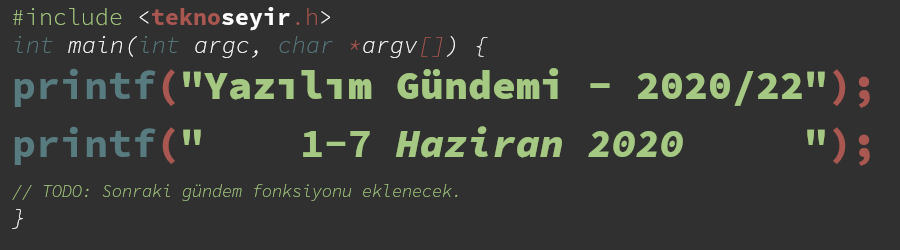
\includegraphics[width=.9\linewidth]{gorseller/yazilim-gundemi-banner.png}
\end{center}

\begin{center}
\href{../21/yazilim-gundemi-2020-21.pdf}{< Önceki Gündem} | \textbf{1-7 Haziran 2020} | \href{../23/yazilim-gundemi-2020-23.pdf}{Sonraki Gündem >}

\href{https://teknoseyir.com/blog/yazilim-gundemi-2020-22}{TeknoSeyir'de Oku}
\end{center}

\section{GitHub, geliştiricileri hedef alan yeni \href{https://securitylab.github.com/research/octopus-scanner-malware-open-source-supply-chain}{bir zararlıyı ortaya çıkardı}: Octopus Scanner}
\label{sec:orga90ca15}
Yazılım gündemi yazıları yazmaya başladığımdan beri sıklıkla geliştiricileri
hedef alan zararlı yazılımların arttığına yönelik haberleri sizlere iletiyorum
fakat bu seferki durum biraz farklı. Mart ayının başlarında GitHub'a \href{https://securitylab.github.com/research/octopus-scanner-malware-open-source-supply-chain}{JJ} takma
isimli güvenlik araştırmacısı GitHub'ı bir güvenlik zafiyeti hakkında uyarıyor
ve GitHub'ın güvenlik takımı harekete geçiyor. Daha önce karşılaştığımız diğer
zararlı yazılım türlerinde saldırganın kendisi kodlarını GitHub'a yükleyip,
yemin yutulmasını beklerken bu sefer zararlı kod bulunan depoların
(repository) sahiplerinin durumdan haberi yok.

\begin{figure}[htbp]
\centering
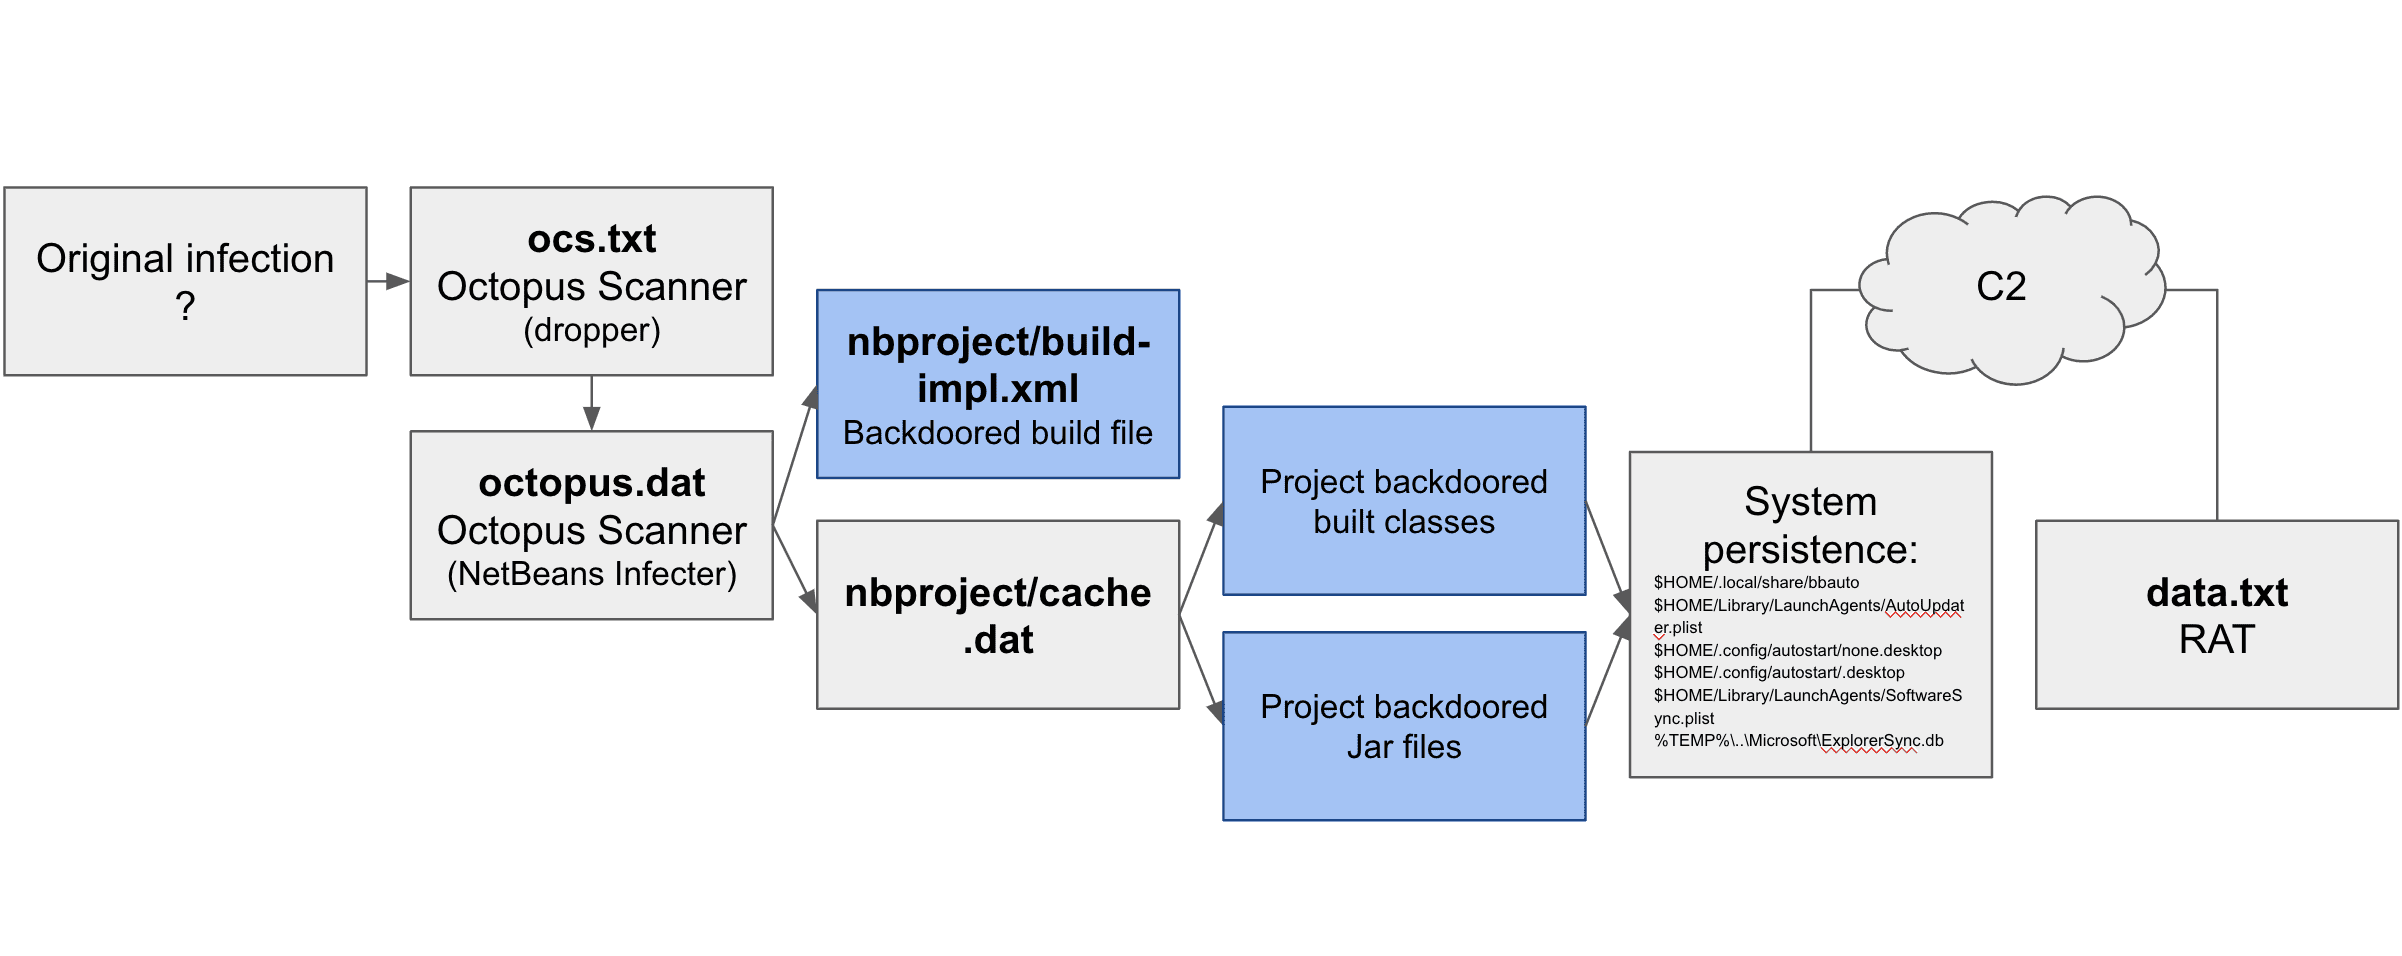
\includegraphics[width=.9\linewidth]{gorseller/github-octopus-scanner.png}
\caption{Zararlı yazılımın bulaşma sistemini gösteren grafik}
\end{figure}

\textbf{NetBeans} ile geliştirilen \textbf{Java} projelerini hedefleyen bu zararlı yazılım,
ilk olarak bilgisayarınızda NetBeans'in kurulu olup olmadığını kontrol ediyor,
eğer kuruluysa bütün NetBeans projelerinize bekiyor ve proje klasörünüzün
içindeki \texttt{nbproject} dizini altına \texttt{cache.dat} isimli bir dosya bırakıyor.
Daha sonra \texttt{nbproject/build-impl.xml} dosyasını düzenleyerek kendisini sizin
geliştirdiğiniz uygulamanın içerisine enjekte ediyor. Oluşturduğunuz JAR
dosyasının içinde bu zararlı yazılım da oluyor. Zararlı yazılım ise
bilgisayarınızda uzak komut çalıştırmaya yarayan bir arka kapı işlevi görüyor.
Ayrıca zararlı yazılım bulaştığı JAR dosyalarının enjekte olmamış hallerini
üretmeyi de önlüyor, yani kendisinin yerine başka bir şey gelmesini
zorlaştırmış oluyor.

GitHub Güvenlik Takımı, bu zararlı yazılımın bulaştığı 26 tane açık kaynaklı
proje tespit etmiş fakat bu projelerin zararlı yazılımdan temizlenmesi biraz
sıkıntılı. GitHub, ilgili repository'lerin sahiplerini bilgilendirerek virüsü
o depolardan temizlese bile kodları bilgisayarına çekmiş olan kullanıcıların
sistemlerinde olan virüs ilgili depolara tekrar kendini kopyalayacak. Takımın
elinde Octopus Scanner zararlısının birkaç varyasyonlu kopyası mevcut fakat
suçlu olmayan kullanıcıları cezalandırmak istemedikleri için şimdilik bir
aksiyon almış değiller fakat geliştiricileri uyarmadan da geçmek istememişler.

Sizler de Java projeleriniz için NetBeans kullanıyorsanız mutlaka
projelerinizdeki \texttt{nbproject} klasörünü kontrol edin. Zararlı yazılım hakkında
daha teknik detaylar için konu başlığına eklediğim blog yazısına göz
atabilirsiniz.
\section{Microsoft Defender SmartScreen, bağımsız \href{https://getimageview.net/2020/06/02/microsoft-defender-smartscreen-is-hurting-independent-developers/}{geliştiricileri zora sokuyor}}
\label{sec:org144d4cd}
Microsoft tarafından geliştirilen Windows 10 işletim sistemiyle birlikte
dağıtılan Microsoft Defender antivirüs yazılımının bir özelliği olan
SmartScreen, bağımsız geliştiriciler tarafından yayınlanan uygulamaları
"tanınmayan" (unknown, unrecognized) olarak işaretlediği için kullanıcılar bu
uygulamaları çalıştırmaya çekiniyorlar.

\begin{figure}[htbp]
\centering
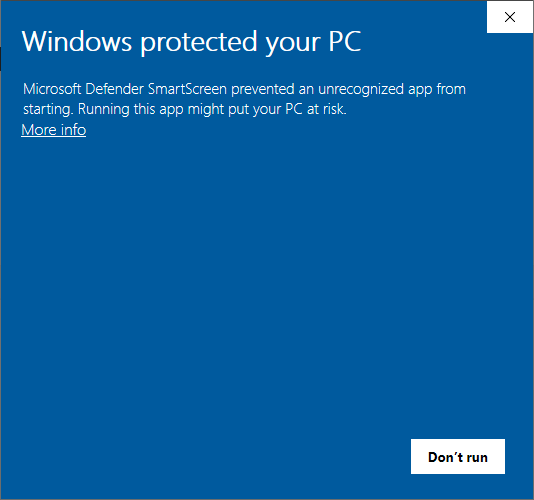
\includegraphics[height=6cm]{gorseller/smartscreen-uyari.png}
\caption{Microsoft Defender SmartScreen tarafından tanınmayan bir uygulamayı açmaya çalıştığınızda gösterilen uyarı penceresi. Yine de uygulamayı çalıştırmak istiyorsanız "More info" yazısına tıklayıp, oradan "run it anyway" düğmesine tıklamanız gerekiyor.}
\end{figure}

SmartScreen'in çalışma mantığını aslında oyunlardaki "itibar" (reputation)
sistemi gibi düşünebiliriz. \texttt{.exe} ile uzantısıyla dağıttığınız uygulamanız ne
kadar kişi tarafından çalıştırılırsa o kadar güvenilir oluyorsunuz. Fakat tek
değerlendirme kriteri bu değil tabii ki, Microsoft aynı zamanda uygulamanın
kim tarafından yayınlandığına da bakıyor fakat bu basit bir "Geliştiren: Eren
Hatırnaz" ifadesinden ibaret değil, tanınmış bir otorite tarafından onaylanmış
bir sertifika almanız ve kodlarınızı bu şekilde imzalamanız gerekiyor. Tahmin
edebileceğiniz gibi ücretsiz bir işlem değil bu. Kod İmzalama Sertifikası
fiyatları sitelere göre değişiklik gösterse de bağımsız geliştiriciler için
uygun denilebilecek bir noktada değil. Üstelik web tarafında ücretsiz SSL
sertifikası sağlayan "Let's Encrypt" gibi bir çözüm de bu tarafta mevcut
değil.

\begin{figure}[htbp]
\centering

\includegraphics[height=7cm]{gorseller/sslcom-code-signing-fiyatlar.png}
\caption{ssl.com sitesinin Kod İmzalama Sertifikasının yıllık fiyatları}
\end{figure}

Bu sertifika ile dağıttınız exe dosyalarını imzalamak maalesef "güvenilir"
olmaya yetmiyor. Çünkü zararlı yazılım geliştiren kişi de aynı şekilde
fiyatını verip, dağıttığı virüsün "güvenilir" sayılmasını sağlayabilir.
Dolayısıyla SmartScreen'in 'itibar' sistemi hala daha geçerli. Exe dosyanız
imzalı olsa bile SmartScreen, daha fazla kullanıcı bu programı çalıştırana
kadar uyarıyı göstermeye devam ediyor. Fakat burada şöyle bir sonsuz döngü de
ortaya çıkıyor: Kullanıcılar uyarı aldığını için programdan şüphelenip
kurmuyorlar, kurmadıkları için SmartScreen, ilgili programın itibar puanını
yükseltmiyor, programın itibarı yükselmediği için de kullanıcılar uyarı mesajı
görmeye devam ediyor.

Üstelik SmartScreen sertifika yenileme işlemini tanımıyor. Yani yeni bir
sertifika aldığınızda tüm bu süreçleri baştan yaşamanız gerekiyor. Bunun da
bir çözümü mevcut fakat bağımsız geliştiriciler için değil, büyük yayıncılar
için mevcut. EV Code Signing Sertifikaları burada devreye giriyor. Yazılım bu
tarz sertifikalar ile bir kere imzalandıktan sonra SmartScreen'den otomatik
olarak geçiyor. Fakat dediğim gibi bu sertifikaların fiyatları bağımsız
geliştiriciler için hiç de ulaşılabilir noktalarda değil.

Sonuç olarak Windows ekosistemi için bağımsız olarak uygulama geliştirmek ve
dağıtmak bir eziyet haline geliyor. Açık kaynak dünyasına iyi bir giriş yapan
Microsoft'un artık Windows ekosistemiyle ilgili bazı şeyleri de tekrar gözden
geçirmesi gerekiyor.

Bu konuda siz ne düşünüyorsunuz? Yorumlar bölümünde konuşalım.
\section{SpaceX Yazılım Takımı, Reddit üzerinde \href{https://www.reddit.com/r/spacex/comments/gxb7j1/we\_are\_the\_spacex\_software\_team\_ask\_us\_anything/}{Soru\&Cevap etkinliği gerçekleştirdi}}
\label{sec:org71b0163}
Bir önceki hafta gerçekleşen başarılı Crew Dragon 2 görevinden sonra gündeme
gelen SpaceX, geçtiğimiz hafta da Reddit üzerindeki \href{https://www.reddit.com/r/spacex/}{/r/spacex} kanalında
yazılım ekibiyle soru \& cevap etkinliği gerçekleştirdi. Binlerce yorum
içerisinden benim gözüme çarpan bazı soruları ve ekibin yazdığı cevapları
sizlere aktarmak isterim.

\begin{itemize}
\item \textbf{Falcon 9 roketinde ve Dragon kapsülünün yazılım tarafında en çok kullanılan
programlama dili nedir? Hangi programlama paradigmalarını kullanıyorsunuz?}
\href{https://www.reddit.com/r/spacex/comments/gxb7j1/we\_are\_the\_spacex\_software\_team\_ask\_us\_anything/ft0aj3b/}{Kaynak}
\begin{quote}
Otonom sistemlerdeki yazılımların tamamı C++ programlama diliyle ve nesne
yönelimli programlama teknikleriyle geliştirildi. Her şeyi mümkün olduğunca
basit tutmaya çalışıyoruz.
\end{quote}

\item \textbf{Uçuş sırasında hata algılama ve hata doğrulama işlerini nasıl
yapıyorsunuz?} \href{https://www.reddit.com/r/spacex/comments/gxb7j1/we\_are\_the\_spacex\_software\_team\_ask\_us\_anything/ft0aj3b/}{Kaynak}
\begin{quote}
Bilgisayarın hesaplamasından kaynaklanabilecek sorunlar için farklı
bilgisayarlar üzerinde aynı hesaplamaları yaptırıyor ve çıktılarını
karşılaştırıyoruz. Sensörlerden kaynaklanabilecek hatalar için de aynı şekilde
birden fazla sensör verisini değerlendiriyoruz. Veri aktarımı sırasında ortaya
çıkabilecek sorunlar için ise aktarılan verilerin içerisine eklenmiş hata
tespit ve hata doğrulama kodlarını kullanıyoruz.
\end{quote}

\item \textbf{Yazılımlarınız küçük küçük parçalardan oluşan bir yapıda mı yoksa her şey
tek bir büyük modül olarak mı geliştiriliyor?} \textbf{(\emph{Kısaca micro service mi,
yoksa mono-repo mu kullanıyorsunuz demek istemiş})} \href{https://www.reddit.com/r/spacex/comments/gxb7j1/we\_are\_the\_spacex\_software\_team\_ask\_us\_anything/ft0aj3b/}{Kaynak}
\begin{quote}
Yazılımlarımız kesinlikle birden çok küçük modülde oluşan bir yapıda. Araçtaki
alt seviye komponentlerden, ara sistemlere kadar her kısımda bir hiyerarşi
mevcut. Farklı alt sistemler genelde birbirlerinden izole edilmiş durumda; bu
izolasyon bazen aynı bilgisayar içerisinde olabilirken, bazen de farklı
bilgisayarlarla sağlanmış izolasyonlar tercih edebiliyoruz.
\end{quote}

\item \textbf{Yazılımlarınızı araçlara yüklemeden önce nasıl test ediyorsunuz?}
\textbf{Falcon/Dragon/Starlink için ne kadar telemetri verisi topluyorsunuz?}
\textbf{Buveriler üzerinde makine öğrenmesi ya da veri analizi yapıyor musunuz?}
\href{https://www.reddit.com/r/spacex/comments/gxb7j1/we\_are\_the\_spacex\_software\_team\_ask\_us\_anything/ft0ahrd/}{Kaynak}
\begin{quote}
Her cihaz için, loop simulator'de olan bir donanıma sahibiz (\emph{anladığım
kadarıyla yazılım ekibinin elinin} \emph{altında sadece geliştirme için kullanılan
cihazın bir kopyası mevcut}). Production ortamına gitmeden önce tüm kodlarımız
bu simülasyonda test edilip sonra asıl aracın içine yükleniyor.

Tipik bir Dragon görevinde yüzlerce GB telemetri verisi topluyoruz. Starlink
cihazlarımız için bu durum 5TB gibi rakamlara ulaşmış durumda. Her uçuştan
sonra, topladığımız tüm verileri gözden geçirip, ilgili cihazın beklediğimiz
gibi çalışıp çalışmadığını kontrol ediyoruz.
\end{quote}
\end{itemize}

Benim okuduklarım içerisinde gözüme çarpan ve aktarmak istediğim sorular ve
cevapları bu şekildeydi (hatalı çevirdiklerim varsa lütfen yorumlar bölümünde
beni uyarın) fakat ilgili reddit gönderisinin altında ilginizi çekebilecek
yüzlerce hatta binlerce soru ve cevap görebilirsiniz. Konu başlığına eklediğim
bağlantıya tıklayarak ilgili gönderiye ulaşabilirsiniz. Eğer sizin ilginizi
çeken başka bir soru ve cevabı varsa yorumlar bölümünde bundan bahsetmeyi
unutmayın.
\section{Tarayıcılara \texttt{:is()} ve \texttt{:where()} CSS \href{https://webplatform.news/issues/2020-06-04}{özelikleri geliyor}}
\label{sec:org1c52d7c}
\href{https://webplatform.news/}{WebPlatform.news} sitesinde geçtiğimiz hafta yayınlanan blog yazısına göre yeni
CSS standartlarından \texttt{:is()} ve \texttt{:where()} artık tarayıcılar tarafından
desteklenecekler. \href{https://webkit.org/blog/10580/release-notes-for-safari-technology-preview-106/}{Safari} ve \href{https://www.fxsitecompat.dev/en-CA/docs/2020/is-pseudo-class-has-been-unprefixed/}{Firefox} bu özelliği implement etmişler, Chromium
ise özellik üzerinde \href{https://bugs.chromium.org/p/chromium/issues/detail?id=568705}{çalışmaya başlamış gözüküyor}. Gelelim bu özelliklerin ne
işe yaradıklarına:

\subsection{\texttt{is()} özelliği}
\label{sec:org68fe7c4}
\texttt{is} (\href{https://developer.mozilla.org/en-US/docs/Web/CSS/:is}{Dokümantasyon}) aslında bir parametre olarak birden fazla CSS selector
kabul edip, içerisindeki seçiciler tarafından seçilebilen herhangi bir
elemanı seçen bir pseudo-class. Cümle biraz karışık oldu farkındayım ama
aşağıdaki örneği inceleyince ne demek istediğini anlayacaksınız. Diyelim ki
elimizde şöyle bir HTML yapısı var:
\begin{minted}[breaklines=true,breakanywhere=true,frame=lines, linenos, label=HTML]{html}
<div class="div1">
  <h1>Selam TeknoSeyir</h1>
</div>
<div class="div2">
  <h1>is() özelliğini</h1>
</div>
<div class="div3">
  <h1>deniyoruz</h1>
</div>
\end{minted}
ve her div'in içerisindeki h1 elemanının yazı rengini kırmızı yapmak
istiyoruz. Önceden bunu şu şekilde yapıyorduk:
\begin{minted}[breaklines=true,breakanywhere=true,frame=lines, linenos, label=CSS]{css}
.div1 h1, .div2 h1, .div3 h1 {
    color:red;
}
\end{minted}
Fakat artık böyle daha sade bir şekilde yazabileceğiz:
\begin{minted}[breaklines=true,breakanywhere=true,frame=lines, linenos, label=CSS]{css}
:is(.div1, .div2, .div3) h1 {
    color: red;
}
\end{minted}
Önceden bu ihtiyacımızı \texttt{:any()} ile giderebiliyorduk fakat onda istediğimiz
düzeyde karışık seçicileri kullanamıyorduk.

\texttt{:where()} özelliği de \texttt{:is()} ile benzer bir yapıya sahip fakat bazı farkları
mevcut. Front-end tarafına pek yakın birisi olmadığı için ne kadar anlamaya
çaba göstersem de farklarını tam olarak anlayamadım o yüzden sizi Mozilla
Developer Network'deki \href{https://developer.mozilla.org/en-US/docs/Web/CSS/:where}{dokümantasyon sayfasına yönlendirmek} durumundayım. Eğer
konu hakkında bilgili arkadaşlar varsa lütfen yorumlar bölümünde bizimle
paylaşsın.
\section{Swift programlama dili topluluğu kendi Paket Kayıt Servisi'ni \href{https://forums.swift.org/t/swift-package-registry-service/37219}{tanımlamayı tartışıyor}}
\label{sec:org903b23e}
Apple tarafından geliştirilen açık kaynak kodlu programlama dili Swift,
geçtiğimiz Haziran ayında GitHub'ın kendi paket kayıt (Package Registry)
servisine \href{https://github.blog/2019-06-03-github-package-registry-will-support-swift-packages/}{eklenmişti}. Fakat bu paket kayıt sisteminin GitHub'ın tekelinde
olmasını istemeyen topluluk üyeleri Swift'in kendi paket kayıt servisini
tanımlaması gerektiği konusunda \href{https://forums.swift.org/t/github-swift-package-management-service/30406}{tartışmalar başlatmıştı}. Geçtiğimiz hafta ise
bu paket kayıt servisini tanılamak için bir \href{https://forums.swift.org/t/swift-package-registry-service/37219}{öneri taslağı ("proposal")
yayınlandı}.

Burada şunu belirtmekte fayda var: Swift programlama dilinin, projedeki
bağımlılıklarınızı yönetebileceğiniz bir paket yönetim aracı zaten var; burada
konuşulan paket \href{https://www.npmjs.com/}{npm} gibi, \href{https://rubygems.org/}{RubyGems} gibi paket kayıt sistemleri. Elbette bu
tartışmaların sonucunda yine bu paket yöneticisine, kendi paket kayıt
servislerimizi ekleme özelliğinin gelmesi planlanıyor.

Swift programlama dilinin forum sayfasında ilgili tartışma devam ediyor.
İlerleyen süreçlerde ne gibi sonuçların çıkacağını hep birlikte göreceğiz.
\section{Go takımı kaynak kodlardaki "\emph{blacklist}", "\emph{whitelist}", "\emph{master}", "\emph{slave}" gibi \href{https://go-review.googlesource.com/c/go/+/236857/}{ifadeleri kaldırdı}}
\label{sec:org9b39113}
Amerika Birleşik Devletlerinde bir polisin siyahi bir vatandaşı öldürmesiyle
başlayan olaylardan sonra ırkçılık konusuyla ilgili var olan hassasiyetlerin
seviyesi de oldukça artmış durumda. Geçtiğimiz hafta içerisinde de Google
tarafından geliştirilen Go programlama dilinin kaynak kodları içerisindeki
"kara liste" ("\emph{siyah liste}"), "\emph{beyaz liste}", "\emph{efendi}" ve "\emph{köle}" gibi
ifadelerin yerini "\emph{allowlist}" ("\emph{kabul listesi}"), "\emph{blocklist}" ("\emph{engel
listesi}"), "\emph{control}" ve "\emph{process}" gibi ifadelere bıraktılar.

Özellikle "\emph{blacklist}" ve "\emph{whitelist}" sadece programlama alanında değil birçok
farklı alanda da artık kalıplaşmış kelimeler olduğu için pek önemli değil gibi
gözükse de biraz düşününce aslında bu değişikliğin mantıklı olduğu ortaya
çıkıyor. En azından bana öyle geliyor. Kaynak kodlardan bu tarz ifadelerin
kaldırılması iyi olmuş bence de.
\section{Yaklaşan Online Etkinlikler}
\label{sec:org0117f32}
\begin{longtable}{|p{9.5cm}|l|}
\hline
Etkinlik İsmi & Tarihi\\
\hline
\endfirsthead
\multicolumn{2}{l}{Önceki sayfadan devam ediyor} \\
\hline

Etkinlik İsmi & Tarihi \\

\hline
\endhead
\hline\multicolumn{2}{r}{Devamı sonraki sayfada} \\
\endfoot
\endlastfoot
\hline
\href{https://kommunity.com/cozumpark/events/cozumpark-sql-tech-talk-live-guvenlik-bakim-ve-performans-363df7aa}{SQL Server Güvenlik, Bakım ve Performans} & 9 Haziran 14:00\\
\href{https://kommunity.com/tracikkaynak/events/acik-seminer-31-gun-devops-ve-micro-frontendler-8b2de35c}{Açık Seminer 31. Gün: DevOps ve Micro Frontendler} & 9 Haziran 14:00\\
\href{https://www.meetup.com/tr-TR/trendyol/events/270950447}{Debezium ile Transaction Log Tailing} & 9 Haziran 18:30\\
\href{https://www.meetup.com/tr-TR/TestHive/events/270909328}{Test Otomasyon Projelerinde Kubernetes Kullanımı} & 9 Haziran 19:30\\
\href{https://kommunity.com/cloud-and-serverless-turkey/events/bulut-cozumlerinde-tasarruf-saglamanin-en-iyi-yontemleri-8b9464e4}{Bulut çözümlerinde tasarruf sağlamanın en iyi yöntemleri} & 10 Haziran 12:00\\
\href{https://kommunity.com/tracikkaynak/events/acik-seminer-32-gun-78318ade}{Açık Seminer 32. Gün: Mikroservis Mimarisi} & 10 Haziran 14:00\\
\href{https://kommunity.com/cozumpark/events/teknoloji-sohbetleri-acik-kaynak-kodlu-yazilimlarla-soc-kurulumu-ve-yonetimi-a7da5264}{Açık Kaynak Kodlu Yazılımlarla SOC Kurulumu ve Yönetimi} & 10 Haziran 14:00\\
\href{https://www.meetup.com/tr-TR/Teknolot/events/270951400}{C\# ve Tensorflow ile Auto Encoder Örneği} & 10 Haziran 14:00\\
\href{https://www.meetup.com/tr-TR/IBMDeveloperTR/events/270784273}{Python ve scikit-learn kullanarak kümeleme algoritmalarına giriş!} & 10 Haziran 15:00\\
\href{https://kommunity.com/ruby-turkiye/events/ruby-turkiye-bulusmasi-8-online-1-7166a878}{Ruby Türkiye Buluşması no.8 Online 1} & 10 Haziran 20:00\\
\href{https://www.meetup.com/tr-TR/GDG-Cloud-Istanbul/events/271074887}{Concurrency 2 - Sohbet Zamanı} & 10 Haziran 21:00\\
\href{https://kommunity.com/devops-turkiye/events/edge-computing-nedir-ve-ne-zaman-kullanilmali-hands-on-demo-7daf47ae}{Edge computing nedir ve ne zaman kullanılmalı?} & 11 Haziran 12:00\\
\href{https://kommunity.com/tracikkaynak/events/acik-seminer-33-gun-mikroservis-tasarim-prensipleri-7d235132}{Açık Seminer 33. Gün: Mikroservis Tasarım Prensipleri} & 11 Haziran 14:00\\
\href{https://kommunity.com/ddd-istanbul/events/event-driven-design-07b35a22}{Event Driven Design} & 11 Haziran 19:00\\
\href{https://kommunity.com/ngturkey/events/state-management-webinar-113474a0}{State Management} & 11 Haziran 20:30\\
\href{https://www.meetup.com/tr-TR/IBMDeveloperTR/events/270949619}{Build your First Microservice based Web Application} & 12 Haziran 14:00\\
\href{https://kommunity.com/devnot-yazilimci-bulusmalari/events/java-net-platformlarinda-microservice-bilesenleri-84d7a825}{Java \& .NET Platformlarında Microservice Bileşenleri} & 12 Haziran 22:00\\
\href{https://www.meetup.com/tr-TR/GDGIstanbul/events/271109645}{Android 11 Beta Launch} & 13 Haziran 19:00\\
\hline
\end{longtable}
\section{Diğer Haberler}
\label{sec:orgfad05de}
\begin{itemize}
\item Apple, parola yöneticisi uygulamalar için \href{https://developer.apple.com/news/?id=06052020a\&1591373342}{yeni kaynaklar yayınladı}. \href{https://github.com/apple/password-manager-resources}{GitHub
Deposu}
\item Atlassian, yeni DevOps \href{https://techcrunch.com/2020/06/02/atlassian-launches-new-devops-features/}{özelliklerini duyurdu}.
\item Microsoft Azure takımı, Azure Maps Creator hizmetini \href{https://azure.microsoft.com/en-us/blog/azure-maps-creator-now-available-in-preview/}{ön izleme olarak
kullanıma açtı}.
\item IBM, MacOs ve iOS için kendi \href{https://www.ibm.com/blogs/research/2020/06/ibm-releases-fully-homomorphic-encryption-toolkit-for-macos-and-ios-linux-and-android-coming-soon/}{şifreleme araç setini duyurdu}. Linux ve Android
için de yakında gelecekmiş.
\item Amazon ve Slack \href{https://www.theverge.com/2020/6/4/21280829/slack-amazon-aws-partnership-amazon-chime-voice-video-calls}{partnerliklerini duyurdular}.
\item AWS, 2. Nesil AMD EPYC işlemcili EC2 C5a \href{https://aws.amazon.com/blogs/aws/new-amazon-ec2-c5a-instances-powered-by-2nd-gen-amd-epyc-processors/}{makinelerini kullanıma açtı}.
\item Git \href{https://lore.kernel.org/git/xmqqzh9mu4my.fsf@gitster.c.googlers.com/}{v2.27.0 sürümü yayınlandı}.
\item PhpStorm \href{https://blog.jetbrains.com/phpstorm/2020/06/phpstorm-2020-2-eap-2/}{2020.2 EAP 2 sürümü yayınlandı}.
\item Rust programlama dilinin \href{https://blog.rust-lang.org/2020/06/04/Rust-1.44.0.html}{1.44.0 sürümü yayınlandı}.
\item MultiCore OCaml projesi için \href{https://discuss.ocaml.org/t/multicore-ocaml-may-2020-update/5898}{Mayıs 2020 raporu yayınlandı}.
\item Blazor WebAssembly \href{https://www.hiddenbrains.com/blog/blazor-webassembly-3-2-0-released.html}{3.2.0 sürümü yayınlandı}.
\item Polaris \href{https://www.fairwinds.com/blog/fairwinds-polaris-1.0-best-practices-for-kubernetes-workloads}{v1.0.0 sürümü yayınlandı}.
\item Wine \href{https://www.winehq.org/announce/5.10}{5.10 sürümü yayınlandı}.
\item Kuesa 3D \href{https://www.kdab.com/kuesa-3d-1-2-release/}{1.2 sürümü yayınlandı}.
\item LibreSSL \href{https://ftp.openbsd.org/pub/OpenBSD/LibreSSL/libressl-3.2.0-relnotes.txt}{3.2.0 sürümü yayınlandı}.
\item TerminusDB \href{https://github.com/terminusdb/terminusdb-server/releases/tag/v2.0.0}{v2.0.0 sürümü yayınlandı}.
\end{itemize}
\section{Lisans}
\label{sec:org5f7347f}
\begin{center}
\begin{center}

\includegraphics[height=1.5cm]{../../../img/CC_BY-NC-SA_4.0.png}
\end{center}

\href{yazilim-gundemi-2020-22.pdf}{Yazılım Gündemi - 2020/22} yazısı \href{https://erenhatirnaz.github.io}{Eren Hatırnaz} tarafından \href{http://creativecommons.org/licenses/by-nc-sa/4.0/}{Creative Commons
Atıf-GayriTicari-AynıLisanslaPaylaş 4.0 Uluslararası Lisansı} (CC BY-NC-SA 4.0)
ile lisanslanmıştır.
\end{center}
\end{document}
